\documentclass[tikz,border=2pt]{standalone}
\usepackage{amsmath}
\usepackage{pgfplots}
\pgfplotsset{compat=1.18}

\begin{document}
% y = 1/x: the product x·(1/x) is always 1, the graph never meets the axes (0 has no reciprocal),
% and reciprocals of numbers between 0 and 1 are larger than 1.
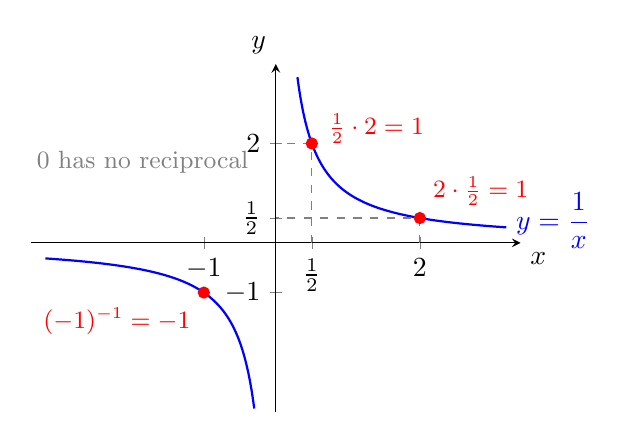
\begin{tikzpicture}
	\begin{axis}[
		axis lines=middle,
		xmin=-3.4, xmax=3.4,
		ymin=-3.4, ymax=3.6,
		xtick={-1,0.5,2}, xticklabels={$-1$,$\tfrac12$,$2$},
		ytick={-1,0.5,2}, yticklabels={$-1$,$\tfrac12$,$2$},
		xlabel={$x$}, ylabel={$y$},
		xlabel style={below right}, ylabel style={above left},
		samples=200, smooth, clip=false,
		width=7.8cm, height=6cm
		]
		\addplot[thick, blue, domain=0.3:3.2] {1/x};
		\addplot[thick, blue, domain=-3.2:-0.3] {1/x};
		\addplot[only marks, mark=*, red] coordinates {(2,0.5) (0.5,2) (-1,-1)};
		\draw[dashed, gray] (axis cs:2,0) -- (axis cs:2,0.5) -- (axis cs:0,0.5);
		\draw[dashed, gray] (axis cs:0.5,0) -- (axis cs:0.5,2) -- (axis cs:0,2);
		\node[red, anchor=south west, font=\small] at (axis cs:2.05,0.55) {$2\cdot\tfrac12=1$};
		\node[red, anchor=west, font=\small] at (axis cs:0.6,2.3) {$\tfrac12\cdot 2=1$};
		\node[red, anchor=north east, font=\small] at (axis cs:-1.05,-1.1) {$(-1)^{-1}=-1$};
		\node[blue, anchor=west] at (axis cs:3.2,0.45) {$y=\dfrac1x$};
		\node[gray, anchor=south, font=\small] at (axis cs:-1.85,1.2) {$0$ has no reciprocal};
	\end{axis}
\end{tikzpicture}
\end{document}
